\documentclass[journal,10pt,onecolumn,compsoc]{IEEEtran} 
    \usepackage[margin=0.75in]{geometry} 
    \usepackage{pdfpages} 
    \usepackage{graphicx}  
    \usepackage{changepage}
    \graphicspath{/images} 
    \usepackage[english]{babel}
    \usepackage{blindtext}
    
    \makeatletter
    \renewcommand{\paragraph}{\@startsection{paragraph}{4}{0ex}%
       {-3.25ex plus -1ex minus -0.2ex}%
       {1.5ex plus 0.2ex}%
       {\normalfont\normalsize\itshape}}
    \makeatother
    \stepcounter{secnumdepth}
    \stepcounter{tocdepth}
    
    \usepackage{tikz}
    \usetikzlibrary{shapes,arrows}
    \tikzstyle{block} = [rectangle, draw, fill=blue!20, 
    text width=5.5em, text centered, rounded corners, minimum height=4em]
    \tikzstyle{subblock} = [rectangle, draw, fill=blue!20, 
    text width=7em, text centered, rounded corners, minimum height=2em]
    \tikzstyle{datablock} = [rectangle, draw, fill=red!20, 
    text width=7em, text centered, rounded corners, minimum height=2em]
    \tikzstyle{line} = [draw, -latex']  
    
    \newenvironment{paddedtikzpicture}{\vspace*{0.5cm}
    \begin{center}\begin{tikzpicture}}
    {\
    \end{tikzpicture}\end{center}
    }  
    \setlength{\parskip}{\baselineskip} \setlength\parindent{24pt}
    \usepackage{url}
    \usepackage{setspace}
    \usepackage{geometry}
    \geometry{textheight=9.5in, textwidth=7in}
    \usepackage{hyperref}
    \usepackage{caption} 
    \usepackage{float} 
    \usepackage{rotating} 
    \usepackage{ragged2e} % provides \RaggedLeft
    \hypersetup{
        colorlinks,
        citecolor=black,
        filecolor=black,
        linkcolor=black,
        urlcolor=black
    }
    \geometry{textheight=9.5in, textwidth=7in}
    \usepackage{listings}
    \usepackage{color}
    \usepackage{cite}
    \definecolor{shadecolor}{RGB}{220,220,220}
    \lstdefinelanguage{JavaScript}{
        keywords={typeof, new, true, false, catch, function, return, null, catch, switch, var, if, in, while, do, else, case, break},
        keywordstyle=\color{blue}\bfseries,
        ndkeywords={class, export, boolean, throw, implements, import, this},
        ndkeywordstyle=\color{darkgray}\bfseries,
        identifierstyle=\color{black},
        sensitive=false,
        comment=[l]{//},
        morecomment=[s]{/*}{*/},
        commentstyle=\color{purple}\ttfamily,
        stringstyle=\color{red}\ttfamily,
        morestring=[b]',
        morestring=[b]"
      }
      \lstset{
        language=JavaScript,
        backgroundcolor=\color{shadecolor},
        extendedchars=true,
        basicstyle=\footnotesize\ttfamily,
        linewidth=7in,
        xleftmargin=.25in,
        showstringspaces=false,
        showspaces=false,
        numbers=left,
        numberstyle=\footnotesize,
        numbersep=9pt,
        tabsize=2,
        breaklines=true,
        showtabs=false,
        captionpos=b
     }
    
    % 1. Fill in these details
    \def \CapstoneTeamName{		The Dream Team}
    \def \CapstoneTeamNumber{		57}
    \def \GroupMemberOne{			Daniel Schroeder}
    \def \GroupMemberTwo{			Aubrey Thenell}
    \def \GroupMemberThree{			Parker Bruni}
    \def \CapstoneProjectName{		A Scalable Web Application Framework for Monitoring Energy Usage on Campus  }
    \def \CapstoneSponsorCompany{	Oregon State Office of Sustainability}
    \def \CapstoneSponsorPerson{		Jack Woods}
    
    % 2. Uncomment the appropriate line below so that the document type works
    \def \DocType{		%Problem Statement
            %Requirements Document
            %Technology Review
            % Design Document
            %Progress Report
            }
            
    \newcommand{\NameSigPair}[1]{\par
    \makebox[2.75in][r]{#1} \hfil 	\makebox[3.25in]{\makebox[2.25in]{\hrulefill} \hfill		\makebox[.75in]{\hrulefill}}
    \par\vspace{-12pt} \textit{\tiny\noindent
    \makebox[2.75in]{} \hfil		\makebox[3.25in]{\makebox[2.25in][r]{Signature} \hfill	\makebox[.75in][r]{Date}}}}
    % 3. If the document is not to be signed, uncomment the RENEWcommand below
    %\renewcommand{\NameSigPair}[1]{#1}
    
    %%%%%%%%%%%%%%%%%%%%%%%%%%%%%%%%%%%%%%%
    \title{Final Report for: \linebreak Scalable Web Application Framework for Monitoring Energy Usage on Campus}
    \author{Daniel Schroeder, Aubrey Thenell, Parker Bruni}
    \date{\today}
    
    \begin{document}
    \maketitle
    \vspace{2cm}
    \begin{center}
    \noindent \textbf{Abstract} \\
                \indent The purpose of this document is to provide final documentation for Group fifty-seven's capstone project. 
    \end{center}         
    
    \newpage
    \pagenumbering{arabic}
    \tableofcontents
        
    % 8. now you write! 
    \section{Introduction to Project}  
    \subsection{Why is this project important?}
    \indent As the population of the world grows exponentially, the demand for energy grows with it. Unfortunately, a massive source of energy for humans comes from non-sustainable fuel burning. This burning releases greenhouse gasses into the earth’s atmosphere, which results in the heating of our planet and many consequences that come as a result. To combat this, communities have decided that it is time to get our energy from more sustainable sources, as well as use it in more sustainable ways. In order to be more sustainable and conscious of our energy consumption, we need to implement modern tools to monitor energy usage data and use that data to make informed decisions on future infrastructure projects. This is necessary to reduce our carbon footprint, reduce costs, and move society to a more sustainable (and eventually fully sustainable) future in regards to energy consumption.

    \indent Oregon State University is revered for its energy efficiency and sustainability and is committed to reducing its carbon footprint through renovations and sustainable consideration with new projects. In this era of technology it is necessary to utilize the tools that are available to us when designing and implementing systems that will increase energy efficiency. Oregon State focuses on reducing its overall costs while supporting a more sustainable environment through less consumption and emissions. With this in mind, OSU has installed energy meters in campus buildings to monitor and record energy data so that it may be analysed by members of Oregon State University’s Sustainability Office. The data that is gathered from these systems can be used to make educated decisions about the current energy usage systems in place, such as monitoring strange fluctuations or anomalies in energy usage in any given building. OSU can address and correct any potential waste from occurring as well as provide a foundation of knowledge to reference when planning future infrastructure projects by utilizing these systems.
    \subsection{Who requested it?}
    \indent Oregon State University's Office of Sustainability previously had contracted a company Lucid to create a web application that acted as an administrative dashboard for monitoring energy use across campus. However, as Oregon State University Sustainability Office scales up its operations and automated reporting, the price of Lucids contract becomes exponentially expensive to maintain. In order to continue data aggregation efforts, the Oregon State Sustainability office has recognized an opportunity for our team to create and plan a project that can take the place of the legacy system. Through creating an EECS capstone project, the Office of Sustainability was able to have an internally sourced web application that can be modified to whichever specifications they desire. It will also save the University hundreds of thousands of dollars that was previously spent on Lucid's services and direct that money towards more sustainable projects for the entire University and help Oregon State reach its carbon neutrality goal of 2025.
    \subsection{Meet the team}
    %%%%% answers the prompts: 
    % Who are the members of your team? 
    % What were their roles?
    % What was the role of the client(s)?} (I.e., did they supervise only, or did they participate in doing development
    \subsubsection{Daniel Schroeder - Developer}
    Daniel was responsible for generating a lot of the front-end data binding implementations with AngularJS. He implement the majority of functionality for all of the main components of the application (blocks, dashboards, stories, buildings). A lot of this process involved finding intuitive ways to query for aggregated data and populate web forms or UI components according to what is needed. A majority of Daniel's contributions revolved around generating a lot of Bootstrap4 and AngularJS webpages that auto-populated drop-down menus, graph data, or user objects so the user could view, create, edit, and delete all of the major components of the application. Additionally, Daniel needed to write route handler functions for and Express.js app that aggregated certain datasets and returned the correct data to the client. 


    \section{Requirements Document}
    %%%%%%% ---------------------------------
    % Insert the requirements document
    %%%%%%% ---------------------------------
    \subsection{Introduction}

    \subsubsection{Purpose}
    The purpose of this document is to outline the project and all associated information. Furthermore, it will outline how the end product will be used, how it was developed, and all resources and documentation referenced and used during development. This document will also describe the application’s target audience, user interface, and any hardware/software requirements. Finally, it will define how our client, team, and users will see the final product and related functionality.
    \subsubsection{Scope}
    This project will provide a web application that displays different collections of energy use reports for campus buildings. Each of these collections will be customizable, with the ability to add, remove, and filter building data according to user preference. The web application will allow users to visually comprehend energy data in a way that can raise awareness about consumption and reduce the campus-wide carbon footprint. The web application will also have three different permission levels: Guest, Registered Users, and Admin Users. Each one will provide permissions to what can be viewed and edited.

    \subsubsection{Definitions, acronyms, and abbreviations} \label{definition}
    \begin{table}[h]
    \centering
    \begin{tabular}{ll}
    \textbf{Term} & \textbf{Definition} \\
    OSU & Oregon State University \\
    MEAN stack & MongoDB, Express, AngularJS, Node.js \\
    JSON & JavaScript Object Notation \\
    AcquiSuite & Data Acquisition Servers responsible for metering energy usage \\
    Collections & User Interface dashboard that displays assortment of blocks \\
    Blocks & Charts/graphs of building data \\
    Stories & Collections of dashboards 
    \end{tabular}
    \end{table}
    \subsubsection{References} 
    The references are: \\

    \tiny
    [1] ``AcquiSuite-A8812'', AcquiSuite | English, 2017. [Online]. Available: \url{http://www.obvius.com/Products/A8812}. [Accessed: 02\-Nov\-2017].

    [2] ``Data-Driven Documents'', D3 | English, 2017. [Online]. Available:  \url{https://d3js.org}. [Accessed: 02\-Nov\-2017].

    [3] ``Vis.js'',Vis.js | English, 2017. [Online]. Available: http://visjs.org/. [Accessed: 02- Nov- 2017].

    [4] ``MongoDB, Express, AngularJS, Node.js'', MEAN.IO | English, 2017. [Online]. Available: http://mean.io. [Accessed: 02- Nov- 2017].

    [5] ``Introducing JSON'', JSON. | English, 2017. [Online]. Available: http://json.org [Accessed: 02- Nov- 2017].

    [6] ``BuildingOS'', BuildingOS | English, 2017. [Online]. Available: https://buildingos.com/. [Accessed: 02- Nov- 2017].

    [7] ``Modbus │How Does Modbus work │Modbus Tutorial│'', Learning Engineering | English, 2016. [Online]. Available: https://www.youtube.com/watch?v=jfKY928Ozrw/. [Accessed: 02- Nov- 2017].

    [8] ``AcquiSuite EMB'', AcquiSuite | English, 2017. [Online]. Available: http://www.obvius.com/Products/A8810-0/. [Accessed: 02- Nov- 2017].

    [9] ``Modbus Addressing \& Wiring Best Practices'', obviusenergy | English, 2017. [Online]. Available: https://www.youtube.com/watch?v=7x0tQf1OsDY. [Accessed: 02- Nov- 2017].

    [10] ``Mocha'', Mocha | English, 2017. [Online]. Available: https://mochajs.org/. [Accessed: 02- Nov- 2017].

    \normalsize
    \subsubsection{Document Overview}
	The remaining sections of this document provide a more elaborate description of product functionality, assumptions, and specific requirements. Section 2 provides information about functional requirements, data requirements, and assumptions made for designing the \textit{Scalable Web Application Framework for Monitoring Energy Usage on Campus}. Section 3 outlines the specific requirements for the final product, the external interfaces that communicate with the software, and the functional requirements of the system.
	
    \subsection{Overall description}
    This section will provide an overview of the web application as a whole, including:
        \begin{enumerate} 
            \setlength\itemsep{1mm}
            \item Details about the user interface and expected user interactions.
            \item An outline of specific constraints and dependences included in development. 
            \item Background information about the specific software requirements.
        \end{enumerate}
    \subsubsection{Product perspective}
    %A block diagram showing the major components of the larger system, interconnections, and external interfaces can be helpful.
    %5.2.1.1 System interfaces
    %This should list each system interface and identify the functionality of the software to accomplish the system
    %requirement and the interface description to match the system.

    This product will replace the current web application that is used by The Oregon State Sustainability Office. The product will display energy usage information about Oregon State University buildings through an intuitive user interface. The application will gather data from energy meters by connecting to AcquiSuite\texttrademark data acquisition servers. The energy data from the meters will be transferred to a database that the product will access directly. Users will interact with the application interface from an internet browser application. 
    
    \subsubsection{Product functions}
    The product will allow users to create accounts that may be given either administrative or user permissions. Users have the ability to personalize their accounts. Administrators accounts will have special capabilities that user accounts will not. \\
    The application will allow users to create customizable dashboards that will contain easily adjustable “blocks” of campus building data that will contain the campus building energy usage data. These “blocks” of data will be the basic building blocks for the dashboard and will provide an intuitive view of the data. They will feature various graph types, building energy efficiency rankings, and data trends.\\
    Each OSU building that contains the energy monitoring meter(s) will have a specific, non-customizable page that will display general information. The product will also have a public interface and a private administrative interface.\\
    Administrators of the application will have the ability to add, remove, or edit entire buildings profiles, building subspaces, or individual meters.
    
    \subsubsection{User characteristics}
    A user that will be using the general public UI will not need to know any specific information about the application to navigate the various energy data presentations. A public user will be able to intuitively navigate the UI at their discretion. \\ 
    An administrative level user will need a basic understanding of the tools of the application because they will be allowed the freedom to control parts of the website as well as have access to more specific energy data within the application. An administrator will likely not need extensive training to use this application for more specific purposes as the administrator UI will be designed to be intuitive to navigate.
    \subsubsection{Constraints}
    Data updates will be limited to a granularity of 15 minute intervals. The data acquisition server is capable of providing a granularity of up to 15 second intervals but it is not necessary for the purposes of the application. Any other constraints on the product are subject to the internet browsing interface that is accessing our product. The UI will be intuitive and able to navigate data presentations, but will not allow manipulation of the data or underlying structure of the application.
    
    \subsubsection{Assumptions and Dependencies}
    The application will be dependant on the data acquisition server. If the data acquisition server is drastically changed or removed, the application will not be functional. Meter data within the application will also be limited by the functionality of the meters themselves. Should a meter malfunction, the energy data will not be gathered which may cause some of the data presentations to deviate from expected data. The use of the application will require a compatible web browsing interface, which may be limited to browsers such as Firefox, Chrome, and Internet Explorer. The functionality of the product will depend on those internet browsers performing as expected with regards to their intended functionality and internet access. 

    \subsubsection{Apportioning of Requirements}
    Future versions of the application may include features such as cost tables, automated electronic invoice generation, energy billing analysis capabilities, budget analysis capabilities, and mobile energy data entry.
    
    \subsection{Specific Requirements}
    
    \subsubsection{External Interfaces}
    AcquiSuite data acquisition servers [meters] made by Obvious
    \begin{itemize}
        \setlength\itemsep{1mm}
        \item Used for collecting electric, water, gas, steam, and other energy parameters over the web.
        \item Data is received through IP-based connection.
        \item Data can be reached anywhere with an internet connection, as long as the AcquiSuite is online.
        \item Data will be collected every 15 minutes.
        \item Data from the AcquiSuite servers will be stored into a database.
    \end{itemize}

    \subsubsection{Functions}
    This section defines how the software system should behave with regards to input and output.
    \begin{itemize}
        \setlength\itemsep{1mm}
        \item The system shall receive and store data from AcquiSuite data acquisition servers into the database. 
        \item The system shall have input validation measures in place to monitor incoming data and protect from malicious injections.
        \item The system shall retrieve data from the database and populate webpages with filtered datasets when prompted.
        \item The system shall have permission based restrictions for accessing certain data.
        \item The system shall generate alerts for offline buildings and high energy usage.
        \item The system shall generate emails for users to access a sign-up form and create an account.
        \item The system shall be able to create arbitrary combinations of datasets given user filters.
        \item The system shall be able to calculate rankings for all the buildings based on certain metrics like ``kilowatt-hour consumption''.
    \end{itemize}

    \subsubsection{Performance Requirements}
    This section describes the functionality requirements for the software as well as what a user should be able to accomplish when using the web application.

    \paragraph{Users}
    The system will have 3 types of users: admin level users, registered users, and generic users. An administrative user will be able to add new meters, buildings, and other objects into the database. A registered user, for example the head of a department, can create their own stories with information and collections that are unique to their own interests or departments. Lastly, a generic user can simply view the publically facing web application and see public dashboards and browse public stories. 
    \begin{itemize}
        \setlength\itemsep{1mm}
        \item A registered user should be able to customize dashboard layouts in a grid-based orientation. A \hyperref[definition]{\textit{story}} page should have a customizable layout where a user can add different \hyperref[definition]{\textit{blocks}} with information relevant to their personal needs.
        \item An administrative user should be able to add buildings to the database through a web form.
        \item An administrative user should be able to add data aquisitions servers.
        \item An administrative user should be able to download specific datasets as a .csv file.
        \item An administrative user should be able to customize public stories.
    \end{itemize}

    \paragraph{Data Management}
    \begin{itemize}
        \setlength\itemsep{1mm}
        \item The web application should update data blocks every 15 minutes as new data is received into the database.
        \item The web application should allow users to create  which are collections of dashboards. These 
        \hyperref[definition]{\textit{stories}} are meant to bring related buildings and datasets together into intuitive groups, for instance ``Residence Halls'' or ``Engineering Buildings.''
        \item The application should be able to filter building data by date range specifications.
        \item The web application should be able to scale up to as many buildings are on campus.
        \item The web application should properly create and store new entities (buildings, users, meters) into the database.
        
    \end{itemize}    

    \paragraph{Visualization}
    \begin{itemize}
        \setlength\itemsep{1mm}
        \item The web application should be able to generate different types of graphs for different \hyperref[definition]{\textit{blocks}}. For example load-profile charts, comparative line charts, and heat maps.
        \item The web application should have generic pages for each building in the database. This page will display a series of graphs and charts that outline energy usage for a particular building.
        \item The \hyperref[definition]{\textit{blocks}} on each page should automatically update as new data is received by the database.
    \end{itemize}
    \paragraph{Objects}
        The system should have three main entities: 
        \begin{itemize}
            \setlength\itemsep{1mm}
            \item \textbf{Building} - A building on campus that is connected to a data acquisition server.
            \item \textbf{Meter} - A specific data acquisition server.
            \item \textbf{User} - A user with a specific role.
        \end{itemize}
        
    \subsubsection{Logical Database Requirements}
    Most of the calls to the database will be requests for meter data from a specific building or group of buildings. Access to the database should be hidden from the user and only accessed from the back-end of the application itself. Any input into the database should be validated and encrypted, if applicable. 
    
    \subsubsection{Design Constraints}
    Design constraints may include server availability which could harm scalability.
    \paragraph{Standards Compliance}
    There may be standards when storing energy data based on The Office of Sustainability Standards.
    [Check with Client]

    \subsubsection{Software System Attributes}
    
    \paragraph{Reliability}
    The system will be reliable at the time of deployment if all data displayed in graphs and charts is correct.
    \paragraph{Availability}
    The system should be consistently available as long as the servers are up and running. As a web application, the system will be available via URL.
    \paragraph{Security}
    The system will validate input for duplicate and malicious content.
    The system will also have back-end functionality to protect user passwords through proper hashing.
    The web application will restrict access to certain pages and content based on user roles and permissions.

    \paragraph{Maintainability}
    Maintainability for this application should be simple for anyone with web development experience. The application code will be organized into logical directories and sub directories that should mimic a full stack web application. There will be documentation that explains how to connect to the AcquiSuite servers and how to use our API for data collection.
    \paragraph{Portability}
    Our web application should be visible and accessible from most web browsers. There are not any host-dependent constraints since it will be hosted from a central server and available to the public via the internet. The source code should stay on Github so modifications can be made easily.
    


include the original document, showing what you thought, at the time, was the project definition with the original Gantt chart
Add (your client should have okay'd): What new requirements were added? What existing requirements were changed? What existing requirements were deleted? Why? 
Add: Final Gantt Chart as a record of what happened when.
    
    \section{Design Document (original)}
    \input{design}
    include the original document, showing what you thought, at the time, was the project design
    Add (your client should have okay'd): What design aspects were changed, deleted or added? Why? 
    \section{Tech Review (original)}
    \subsection{Daniel Technology Review Overview}
\subsubsection{Introduction}
My role in this project will be integrating the front-end with the back-end framework and acting as a dev ops engineer. I want to take on the role of dev ops for this project to hone in on certain skills that have not previously been targeted in my past web-development internships. I have created UX/UI and built pages/forms that  manipulate database data. I have written back-end model functions to retrieve data for use in an application. Now I want to manage the full-fledged construction of a full stack web application. Another motive for taking a dev ops role is with a framework like NodeJS, there are endless amounts of libraries and frameworks that you can utilize in your application that can simplify every component. What I want to take away from this course is a well-rounded knowledge about how different components of an application work together and how to integrate each part efficiently.\\
By taking a dev ops role in this project, I will be able to:
\begin{itemize}
    \item Transition away from the tasks I've been previously trained on.
    \item Help my teammates understand things that I have previously learned by not implementing them myself.
    \item Develop a more comprehensive understanding of NodeJS, Angular, Express, and NOSQL Databases.
    \item Take lead in developing a high-end development environment for my team and I in order to create efficient workflow.
    \item Implement components of our web application that are new to me.
\end{itemize}

There are a lot of different components that go into making a web application work and it takes a high-level understanding to implement them all. Our web application will act like an admin dashboard that displays specific charts and graphs based on user preference.\\
Firstly, from a dev ops perspective, we need an architecture that can host a NodeJS application from a single VM. We will be using Amazon Elastic Compute Cloud (EC2) to host our web server. This EC2 instance will listen for inbound requests and transfer them to our Node server daemon. Our Node server will then have to communicate with our MongoDB to retrieve the necessary data.\\
Secondly, we will need a workflow architecture for continuous deployment that can be utilized by all members of the team. We will use Github to create a ``Git-flow'' environment that proceeds as follows:
\begin{itemize}
    \item The repository master branch is considered to be ``production.''
    \item Developers will create ``feature branches'' branched from master.
    \item Feature branches will be pull requested, reviewed, and merged into the master branch.
\end{itemize}
Git-flow allows team members to work on separate features while building off of the current working application. Feature branches make sure that the master branch is always in working condition and no new code gets merged without review and confirmation that it works.\\
Thirdly, our web application also has users with different roles, which adds a lot of overhead to the application. Our application needs to have user authentication, user sessions, user roles, and code to enforce it all. Using Google's oAuth 2.0 authentication, our application will force users to log in with their Google accounts and Google will handle most of the overhead. When a user logs in, ``the Google Authorization Server sends [the] application an access token'' which is then stored in the database instead of a user password \cite{oauth}. Then, through utilizing the Passport.js authentication middleware, we can create user sessions and manage authentication with this Google token and not have any security issues with passwords.\\
The final main component of our web application is the actual functionality of providing data visualizations to the user in a clean and dynamic way. This will include retrieving and parsing data from Acquisuite data acquisition servers, storing this information in the database, and creating dynamic graphs and charts using a visualization framework that can be manipulated by the user. This will involve developing filters and date ranges that can be applied to all the data to select sub-portions of data based on specific buildings, collections of certain buildings, or time periods. Having a visualization framework that works well with AngularJS and our MongoDB database is essential in creating a smooth, dynamic web application. 
%%%%%%%%%%%%%%%%%%%%%%%%%%%%%%%%%%%%%%%%%%%%%%%%%%%%%%%%%%%%%%%%%%
%%%%%%%%%%%%%%%%%%% Visualization Frameworks %%%%%%%%%%%%%%%%%%%%%
%%%%%%%%%%%%%%%%%%%%%%%%%%%%%%%%%%%%%%%%%%%%%%%%%%%%%%%%%%%%%%%%%%
\subsubsection{Visualization Frameworks}
Our web application will provide near-real time data visualizations for energy consumption by buildings on campus. This application will need to dynamically create charts and graphs based on energy data from the database. A key to choosing a visualization library will be to find one that can be dynamically created and changed as new data is received from the data acquisition servers, and the ability to create chart templates that can be reused on multiple pages with different input parameters.\\
\textbf{Basic Criteria}
\begin{itemize}
\item Handle dynamic data. 
\item Allow the user to manipulate data by applying filters or selecting data points. 
\item Works well with Angular framework.
\item Templatable.
\end{itemize}
\paragraph{D3.js}
%https://www.dashingd3js.com/d3-resources/d3-and-angular
\textit{Repository Commits: 4,104}\\  
\textit{Contributors: 120}\\
D3 allows you to bind arbitrary data to a Document Object Model (DOM), and then apply data-driven transformations to the document \cite{d3_home}. It is extremely well documented and widely used. D3 has a high learning curve for beginners to take head-on, but has a wide array of different visualizations and customization.\\
\textbf{Pros}
\vspace{-0.5cm}
\begin{itemize}
\item A lightweight, versatile javascript library that uses ``SVG to create the graphical elements'' and appends them to DOM elements \cite{Schwartz}. 
\item Makes use of javascript functions and DOM controlling functionality to dynamically change the content of the page. 
\item Provides a lot of variety and ability to customize graphics.
\item Widely used and there is a lot of documentation and resources available to assist the learning and development processes.
\end{itemize}
\textbf{Cons}
\vspace{-0.5cm}
\begin{itemize}
\item D3 is essentially an API to to manipulate SVG, it is not a charting library in of itself \cite{Sun}.
\item You cannot easily pass a data set into a specified chart type like other libraries.
\item A large amount of ``up-front investment in time to get a handle on the D3 language''\cite{Jacobson}.
\item Angular and D3 both attempt to control the DOM and so you have to find a way to make the two work together which is counter intuitive to both framework's APIs. 
\end{itemize}
\paragraph{Vis.js}
\textit{Repository Commits: 3,165}\\
\textit{Contributors: 137}\\
Vis.js is a lightweight charting library that allows users to create clean charts from dynamic data sets \cite{vis}. It is responsive and allows for interaction with the data on the page. Vis.js is praised for it's network chart capabilities but is limited in the number of different modules you can create.\\
\textbf{Pros}
\vspace{-0.5cm}
\begin{itemize}
\item Easy to use and less of a learning curve than D3.
\item Allows for interaction and manipulation of data on the chart.
\item Able to handle large amounts of dynamic data.
\item Really clean and nice looking graphics.
\end{itemize}
\textbf{Cons}
\vspace{-0.5cm}
\begin{itemize}
\item Limited amount of possible chart types.
\item Does not have built in heat map.
\end{itemize}
\paragraph{Chart.js}
\textit{Repository Commits: 2,465}\\ 
\textit{Contributors: 236}\\
Chart js is a very lightweight library that provides 6 chart types and fully responsive designs. ChartJS is well documented and easy to use, but lacks in variety.\\
\textbf{Pros}
\vspace{-0.5cm}
\begin{itemize}
\item Uses HTML5 canvas element.
\item Allows for easy creating based on chart type specification.
\item Library provides Line Charts, Bar Charts, Radar Charts, Pie Charts, Polar Area Charts, and Doughnut Charts.
\item Very responsive charts based on screen width.
\item Simple API, easy to use.
\end{itemize}
\textbf{Cons}
\vspace{-0.5cm}
\begin{itemize}
\item Limited amount of possible chart types.
\item Does not have built in heat map.
\end{itemize}
\paragraph{Conclusion}
In conclusion, despite the steep learning curve associated with D3.js we think it will be the best option for our web application. It has the widest range of available graphs to accommodate all the client's requirements and desired visualizations. There are also a number of wrapper libraries available for D3.js like DC.js and dimple.js to help create charts from D3. This is a great way to get around the inconveniences and downsides to D3.js and reap the benefits of all the other charting libraries. Another benefit to using D3 is the extensive amount of templates, examples, and documentation that exists to help guide the process and implementation of our application.\\
It is possible that our decision will change as we begin creating the web application and find other libraries to fit our needs. There are a lot of AngularJS libraries that specify unique directives for implementing different charting libraries and we might find one throughout the midst of our development that handles all of our needs swiftly and effectively. One of the main factors that guided our decision towards D3 was the ability to create heatmaps, which was a client requirement. If this requirement falls through, or we simply use D3 only for heatmaps, we may be able to implement a more lightweight charting library to achieve better simplicity.
%%%%%%%%%%%%%%%%%%%%%%%%%%%%%%%%%%%%%%%%%%%%%%%%%%%%%%%%%%%%%%%%%%
%%%%%%%%%%%%%%%%%%%%%%%% Authentication %%%%%%%%%%%%%%%%%%%%%%%%%%
%%%%%%%%%%%%%%%%%%%%%%%%%%%%%%%%%%%%%%%%%%%%%%%%%%%%%%%%%%%%%%%%%%
\subsubsection{Means of Incorporating Authentication}
Our web application will have an authentication layer which will allow users to register for our application and design their own ``stories.'' Our application will also authenticate user roles so that administrative users will have access to exclusive parts of the application. We want a simple way of authenticating users, while keeping personal information safe.\\
\textbf{Basic Criteria}
\begin{itemize}
\item Remember users across web pages (sessions). 
\item Allow users to be added to the database. 
\item Protect sensitive information like passwords.
\end{itemize}
\paragraph{Building Our Own Authentication Layer}
Node.js has a lot of helpful modules and packages that allow you to create your own password hashing functions and generate a custom authentication layer. There is a ``crypto'' module that is included in Node.js that ``provides cryptographic functionality that includes a set of wrappers for OpenSSL's hash, HMAC, cipher, decipher, sign and verify functions''\cite{Crypto}. In addition to the crypto module, there are numerous Node.js extension modules that perform different hashing functions and provide the same functionality as the native crypto module. There are modules like \href{https://www.npmjs.com/package/bcrypt-Node.js}{\textit{bcrypt}} and \href{https://www.npmjs.com/package/scrypt}{\textit{scrypt}} that use different hashing algorithms to salt and hash password into a fixed length string to be stored into the database. 

\noindent\textbf{\textit{\hyperref[sec:node_crypto]{\textcolor{red}{link: See Appendix A for code listing}}}} \\

\noindent\textbf{Pros}
\vspace{-0.5cm}
\begin{itemize}
    \item Creating our own authentication layer would provide us full control over how passwords are hashed and stored into the database. 
    \item Provide understanding of every component that goes into our application's authentication.
    \item Do not have to rely on another API to authenticate users.
\end{itemize}
\textbf{Cons}
\vspace{-0.5cm}
\begin{itemize}
    \item Laborious work and very time consuming.
    \item A lot of room for error and the possibility of data being compromised.
\end{itemize}
\paragraph{Outsourcing Authentication to Google}
Google oAuth 2.0 is a Google API that authenticates users by signing in with their google accounts. There is a lot of documentation about how to integrate Google's authentication API with Node.js. \href{http://www.passportjs.org/}{\textit{Passport}} is authentication middleware for Node.js that provides simple authentication using ``A comprehensive set of strategies support authentication using a username and password, Facebook, Twitter,'' and Google \cite{passport}.

\noindent\textbf{\textit{\hyperref[sec:passport_oauth]{\textcolor{red}{link: See Appendix A for code listing}}}} \\

\noindent\textbf{Pros}
\vspace{-0.5cm}
\begin{itemize}
    \item Takes all the security risks out of creating our own authentication.
    \item Saves a lot of development time. 
    \item Widely used with a lot of documentation.
    \item Relieves the need to store user passwords in the database.
    \item Can use the passport authentication middleware to simplify authentication even further.
\end{itemize}
\textbf{Cons} 
\vspace{-0.5cm}
\begin{itemize}
    \item Limits users to having a google account.
    \item Relies on Google API to be working and running.
    \item Adds dependencies to the project.
\end{itemize}
\paragraph{Use CAS (Central Authentication Service)}
CAS is an authentication process that redirects users to a CAS login page like the one that Oregon State University uses for most things like Canvas, Box, and MyDegrees.\\

\noindent CAS uses sessions and a CAS Client server to authenticate users throughout a web application:
\textit{When CAS redirects the authenticated user back to your application, it will append a \{ticket\} parameter to your url.}
\noindent The ticket returned to your application is opaque, meaning that it includes no useful information to anyone other than the CAS Server. The only thing that your application can do is send this ticket back to CAS for validation.
CAS will then either respond that this ticket does not represent a valid user for this service, or will acknowledge that this ticket proves authentication. In the later case, CAS will also supply the user's NetID so that you know the identity of the user \cite{how_cas_works}.

\noindent\textbf{Pros} 
\vspace{-0.5cm}
\begin{itemize}
    \item Can use the OSU official CAS to provide a nice theme.
    \item Keeps the same centralized CAS server as the rest of Oregon State University's application.
\end{itemize}
\textbf{Cons}
\vspace{-0.5cm}
\begin{itemize}
    \item Relies on Oregon State University's CAS server to be operational. 
    \item Adds extraneous code and implementation.
    \item Not as modular as the Node.js/Passport implementations of oAuth 2.0.
\end{itemize}
\paragraph{Conclusion}
After reviewing the different means of including authentication for our web application, we think that using the Passport middleware to implement Google's oAuth 2.0 API would be the best option. It can be easily integrated into Node.js applications, everyone at Oregon State University has a Gmail account, and it removes the need to store any passwords into our database. The Google oAuth 2.0 authentication process uses a token that is received from the Google API that we will store along with the user ID and name into our database.\\
Another large benefit to using the Passport.js and Google oAuth 2.0 authentication process is that passport handles most of the overhead involved with user sessions and per-page authentication. Using a small cookie set that contains the user id, ``Passport will serialize and deserialize user instances to and from the session'' to handle login sessions throughout the application \cite{passport_session}.

\noindent\textbf{\textit{\hyperref[sec:passport_session]{\textcolor{red}{link: See Appendix A for code listing}}}} \\

\noindent Using Google authentication and the Passport middleware will drastically simplify the authentication process of our application and keep the amount of sensitive data in our database to a minimum.
%%%%%%%%%%%%%%%%%%%%%%%%%%%%%%%%%%%%%%%%%%%%%%%%%%%%%%%%%%%%%%%%%%
%%%%%%%%%%%%%%%%%%%%% Front-end Framework %%%%%%%%%%%%%%%%%%%%%%%%
%%%%%%%%%%%%%%%%%%%%%%%%%%%%%%%%%%%%%%%%%%%%%%%%%%%%%%%%%%%%%%%%%%
\subsubsection{Front-end Framework}
Our web application will be a series of dashboards to display energy data based on different buildings and subsets of buildings on Oregon State University's campus. A key part to designing a clean dashboard is having a well-spaced grid-like layout with different charts and graphs to display a multitude of different data sets and trends. Rather than customizing classic html elements and using div containers to space our dashboard, we wanted to look into bootstrapped dashboard templates that allow easy customization and clean-looking results.\\ 
\textbf{Basic Criteria}
\begin{itemize}
\item Integrates well with Angular and the entire MEAN stack. 
\item Components can be easily integrated with Visualization Framework. 
\item Customizeable.
\end{itemize}
\paragraph{CSS Bootstrap}
\textit{Repository Commits: 17,255}\\ 
\textit{Contributors: 953}\\
CSS Bootstrap is the most widely used CSS framework available. It has the most expansive component list and helps developers create clean and beautiful UX/UI in minimal time frames. Bootstrap allows developers to get their publications up and running quickly without having to worry about front-end styling. A major issue with Bootstrap is that it tends to look very similar across applications and leaves little room for simple customization.\\
\vspace{-0.5cm}
\noindent\textbf{\textit{\hyperref[sec:ui_bootstrap]{\textcolor{red}{link: See Appendix A for code listing}}}} \\

\noindent\textbf{Pros}
\vspace{-0.5cm}
\begin{itemize}
    \item Extensive component list, responsive design, and built-in Javascript functions.\cite{puranjay_2015}
    \item EFully responsive design.
    \item Huge developer contribution and maintenance.
    \item Used by major companies like Lyft.com, Vogue.com, Vevo.com, and Newsweek.com. \cite{puranjay_2015}
\end{itemize}
\textbf{Cons}
\vspace{-0.5cm}
\begin{itemize}
    \item Unsuitable for small scale projects. \cite{puranjay_2015}
    \item Not good if you want to have large control over UI.
\end{itemize}
\paragraph{Pure CSS}
\textit{Repository Commits: 541}\\ 
\textit{Contributors: 51}\\
Pure CSS is known for its lightness and simplicity. Because it's small, it is very fast loading and makes for a lightweight web application. It is also unique in that it allows modules/components to be downloaded individually, reducing its size even more. Pure CSS is good for small projects that need to get up and running quickly and easily.\\

\noindent\textbf{Pros}
\vspace{-0.5cm}
\begin{itemize}
    \item Meant for small project to get up and running quickly.
    \item Responsive design by default.
    \item Pure CSS is modular so you can download only the components you need.
    \item The complete module is very small so it is quick loading.
    \item Able to be used complimentary with other frameworks.
\end{itemize}
\textbf{Cons} 
\vspace{-0.5cm}
\begin{itemize}
    \item Not as extensive component list as Bootstrap.
\end{itemize}
\paragraph{Foundation}
\textit{Repository Commits: 15,094}\\ 
\textit{Contributors: 959}\\
Framework is the second most popular css framework on the market behind Bootstrap and tends to perform just as well. Unlike bootstrap's very prominent theme, Foundation allows for more customization with the look and feel of web pages \cite{Nick_Pettit}. Foundation also has a very good grid system to make the layout of components clean and responsive \cite{blankenship_2017}.\\ 

\noindent\textbf{Pros}
\vspace{-0.5cm}
\begin{itemize}
    \item Responsive design by default.
    \item Easier to customize than Bootstrap.
    \item CSS classes are built in. \cite{team_2015}
    \item More unique look than the more-popular Bootstrap.
    \item Good grid implementations with customizable grid layouts.
\end{itemize}
\textbf{Cons}
\vspace{-0.5cm}
\begin{itemize}
    \item Less maintained than Bootstrap.
    \item Lack of support.
    \item Higher learning curve than Bootstrap.
\end{itemize}
\paragraph{Conclusion}
A lot of online resources acknowledged the fact that it is hard to make a website not look like Bootstrap when using Bootstrap css. Despite this, we are choosing to use Bootstrap as the main front-end framework for our application. Similar to our reasoning behind choosing D3.js, we would like to use a framework that is heavily supported and well-documented, as it will be easier to answer questions during development. We think that the time spent restyling Bootstrap to make it look unique will not compare to the time saved by utilizing a well-documented framework. There is also a project called \href{https://angular-ui.github.io/bootstrap/}{UI Bootstrap} that works with AngularJS to create directives for each of the Bootstrap components \cite{sevilayha_2015}.

    \section{Weekly Blog Posts (all team members' posts)}
    \subsection{Daniel Blog Posts}
    \input{daniel_blogs}
    formatted nicely and clearly distinct from one another
    include all members posts, clearly distinct, clearly organized
    \section{Final Poster}
    %--------------- include image poster
    %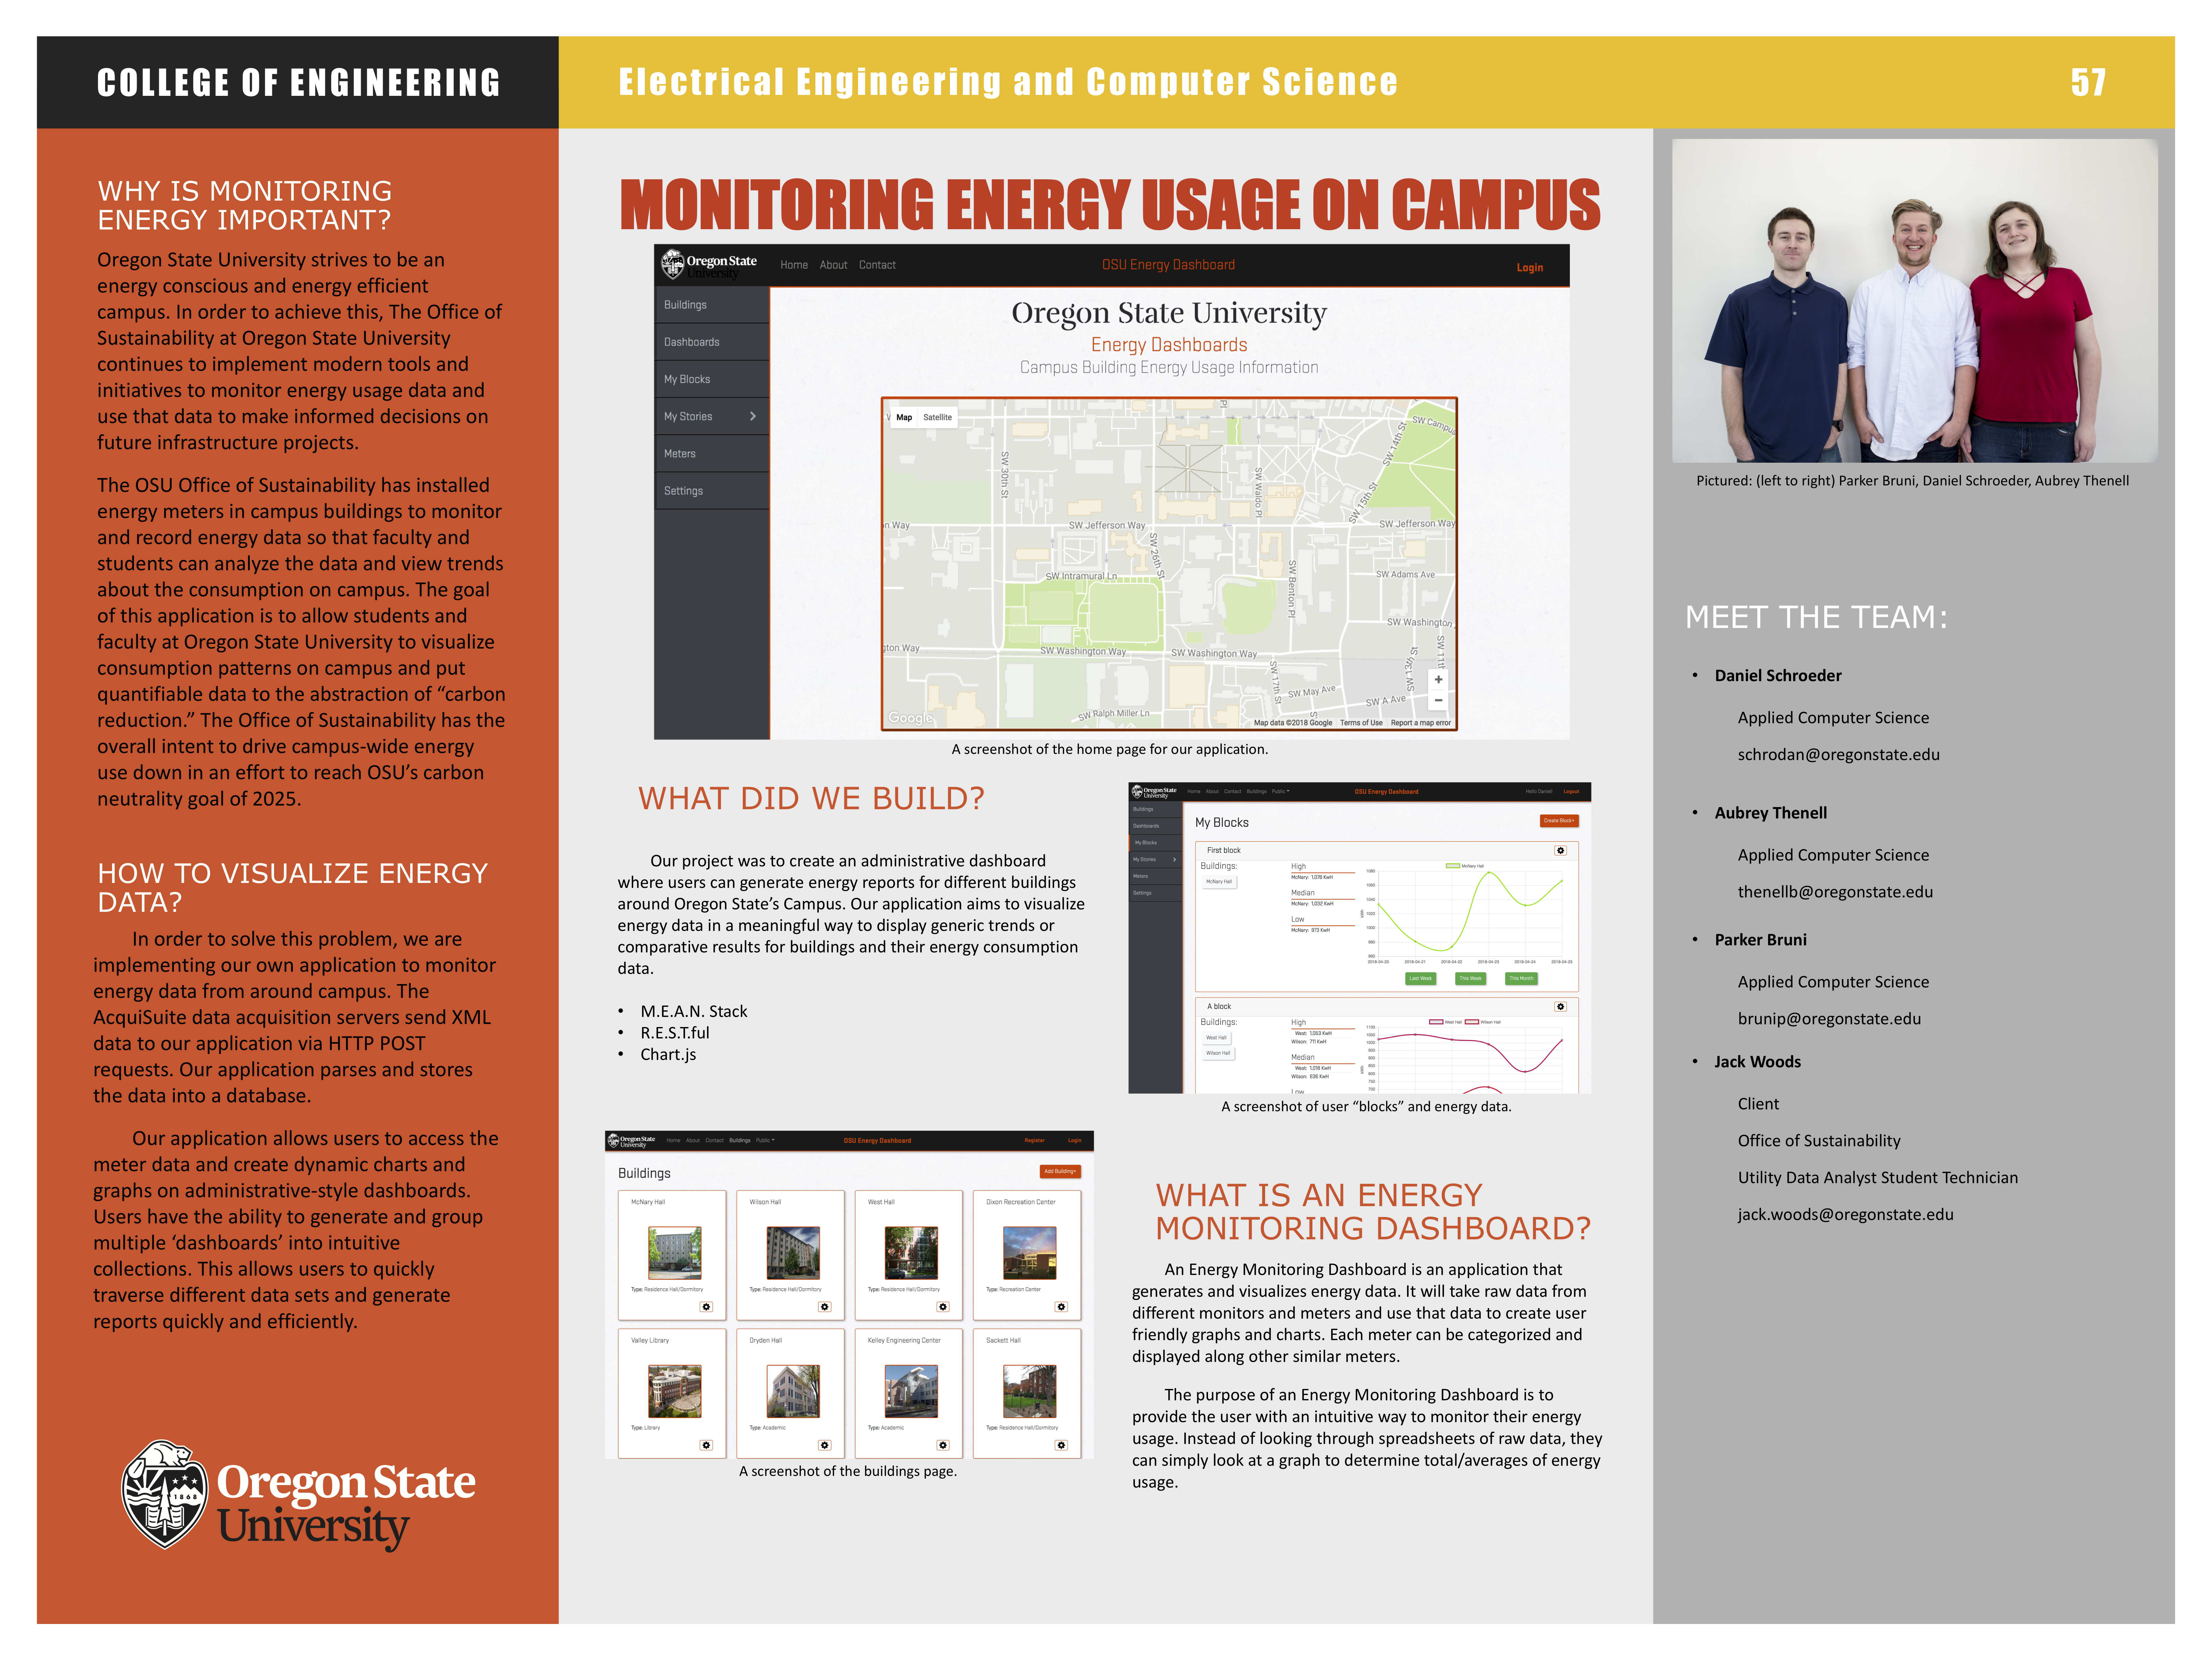
\includegraphics[angle=270,origin=c,width=18cm]{images/poster1} 
    \section{Project Documentation}
    \subsection{How does your project work? (Could include the following...)}
    \begin{itemize}
    \item What is its structure?
    \item What is its Theory of Operation?
    \item Block and flow diagrams are good here.
    \end{itemize}
    \subsection{How does one install your software, if any?}
    \subsection{How does one run it?}
    \subsection{Are there any special hardware, OS, or runtime requirements to run your software?}
    \subsection{Any user guides, API documentation, etc.}
    This needs to be detailed enough to recreate and/or use your project!
    \section{Recommended Technical Resources for Learning More}
    What web sites were helpful? (Listed in order of helpfulness.)
    What, if any, reference books really helped?
    Were there any people on campus that were really helpful?
    \section{Conclusions and Reflections (each team member answers all questions individually)}
    \subsection{Daniel}
    \subsubsection{What technical information did you learn?}    
    Before building this project, I had very little (if any) knowledge about AngularJS as a front-end framework, MongoDB, Amazon web services, or Express.js. While I had previously tried to do small scale M.E.A.N. stack applications, they were always bootstrapped from an example code source and I never truly understood the fundamentals behind a RESTful API or a full stack web application. I think building this project allowed me to really learn 3 main concepts:
    \begin{itemize}
        \item Read and learn from documentation
        \item Reach proficiency with the M.E.A.N. stack frameworks
        \item Understand how to design and implement a large software architecture
    \end{itemize}
    This was my first project built from scratch of something to this size and scale and it taught me a lot about the design process. I now understand why it is so common for companies to migrate legacy monolith architectures into smaller microservices. Systems that are extremely large become easily cluttered and become filled with minute work-arounds or case-dependent implementations that are not good for readability or robustness. I found that we lacked a large amount of understanding during the design process and it made a huge impact during the implementation of our project.
    \subsubsection{What non-technical information did you learn?}
    The biggest non-technical skill I learned during the course of this project was time-management and team-management. Towards the end of the project, I began setting myself hard deadlines for feature completion and implementation which proved to be extremely helpful for finishing everything that needed to get done. During the winter term, I would pick away at something here, do a little bit on something there, but never set myself deadlines for finishing up concrete requirements. I found myself becoming more and more relaxed with finishing up code and that made me fall behind at the start of spring term. I think better planning with both the architecture design and Gantt chart/read map would have proven extremely helpful throughout the development of this project.
    \subsubsection{What have you learned about project work/project management?}
    Planning and sharing work to ensure completion is crucial. Towards the end of the project, I found myself assigning personal tasks and tasks to group members with hard deadlines to speed up completion. Prior to having concrete due dates for features, the rate of implementation was slow and it seemed we were always crunched for time. I think breaking the project up into small pieces and following a concrete road map for implementations would have proven extremely helpful. 
    \subsubsection{What have you learned about working in teams?}
    I think it is important to lay out your values and expectations of yourself and others at the beginning of the project. I found that my expectations for quality and time-management differed from my group members. Putting this on the table and discussing what everyone expects from each other I think would have reduced a lot of that uncertainty and frustration throughout the year. 
    \subsubsection{If you could do it all over, what would you do differently?} 
    There are specific technical changes I would make to this project if I could do it all over again. First and foremost, for the amount of relations we had in our data, I think using MySQL as a back-end would have benefitted us immensely. Secondly, and as mentioned above, I think that a thorough Gantt chart and implementation roadmap would have assisted the flow and overall quality of the project. If we had a lot of the necessary backend requirements or charting implementations done sooner, it would have alleviated a lot of the debigging and error testing that was needed towards the end of the project. I would have also like to have everyone working on and understanding every aspect of the project. Learning curves and skill-level limitations played a large role in preventing contributions in many areas of the project.
    \subsection{Parker}
    \subsubsection{What technical information did you learn?}    
    \subsubsection{What non-technical information did you learn?}
    \subsubsection{What have you learned about project work?}
    \subsubsection{What have you learned about project management?}
    \subsubsection{What have you learned about working in teams?}
    \subsubsection{If you could do it all over, what would you do differently?} 
    \subsection{Aubrey}
    \subsubsection{What technical information did you learn?}    
    \subsubsection{What non-technical information did you learn?}
    \subsubsection{What have you learned about project work?}
    \subsubsection{What have you learned about project management?}
    \subsubsection{What have you learned about working in teams?}
    \subsubsection{If you could do it all over, what would you do differently?} 
    \section{Appendix 1: Essential Code Listings.}
    You don't have to include absolutely everything, but if someone wants to understand your project, there should be enough here to learn from. If you worked within a larger project, something like a patch file might be a good way to go.
    \subsubsection{Node.js crypto salt/hash password example}
\label{sec:node_crypto}
\begin{lstlisting}[
caption={[An example of how to salt hash passwords using the Node.js crypto module]An example of how to salt hash passwords using the Node.js crypto module (Taken from \href{https://ciphertrick.com/2016/01/18/salt-hash-passwords-using-Node.js-crypto/}{\textit{Rahil Shaikh's example}})\cite{Rahil_Shaikh}}
]
'use strict';
var crypto = require('crypto');
/**
    * generates random string of characters i.e salt
    */
var genRandomString = function(length){
    return crypto.randomBytes(Math.ceil(length/2))
            .toString('hex') /** convert to hexadecimal format */
            .slice(0,length);   /** return required number of characters */
};
/** hash password with sha512.
    * @function
    * @param {string} password - List of required fields.
    * @param {string} salt - Data to be validated.
    */
var sha512 = function(password, salt){
    var hash = crypto.createHmac('sha512', salt); /** Hashing algorithm sha512 */
    hash.update(password);
    var value = hash.digest('hex');
    return {
        salt:salt,
        passwordHash:value
    };
};
function saltHashPassword(userpassword) {
    var salt = genRandomString(16); /** Gives us salt of length 16 */
    var passwordData = sha512(userpassword, salt);
    console.log('UserPassword = '+userpassword);
    console.log('Passwordhash = '+passwordData.passwordHash);
    console.log('nSalt = '+passwordData.salt);
}
\end{lstlisting}
\subsubsection{Using Passport.js to include Google oAuth 2.0 authentication}
\label{sec:passport_oauth}
\begin{lstlisting}[
caption={[Using passport to include Google oAuth 2.0 authentication]Using passport to include Google oAuth 2.0 authentication. (Taken from \href{http://www.passportjs.org/docs/username-password}{\textit{Passport Documentation}})\cite{passport_doc}}
]
var passport = require('passport');
var GoogleStrategy = require('passport-google-oauth').OAuth2Strategy;

// Use the GoogleStrategy within Passport.
//   Strategies in Passport require a `verify` function, which accept
//   credentials (in this case, an accessToken, refreshToken, and Google
//   profile), and invoke a callback with a user object.
passport.use(new GoogleStrategy({
    clientID: GOOGLE_CLIENT_ID,
    clientSecret: GOOGLE_CLIENT_SECRET,
    callbackURL: "http://www.example.com/auth/google/callback"
    },
    function(accessToken, refreshToken, profile, done) {
        User.findOrCreate({ googleId: profile.id }, function (err, user) {
            return done(err, user);
        });
    }
));
\end{lstlisting}    
\subsubsection{Using Passport.js to maintain user sessions.}
\label{sec:passport_session}
\begin{lstlisting}[
caption={[The user ID is serialized to the session, keeping the amount of data stored within the session small. When subsequent requests are received, this ID is used to find the user, which will be restored to req.user.]The user ID is serialized to the session, keeping the amount of data stored within the session small. When subsequent requests are received, this ID is used to find the user, which will be restored to req.user. (Taken from \href{http://www.passportjs.org/docs}{\textit{Passport Documentation}})\cite{passport_session}}
]
passport.serializeUser(function(user, done) {
    done(null, user.id);
    });
    
    passport.deserializeUser(function(id, done) {
    User.findById(id, function(err, user) {
        done(err, user);
    });
    });
\end{lstlisting}

\subsubsection{Using UI Bootstrap to create a datepicker object.}
\label{sec:ui_bootstrap}
\begin{lstlisting}[
    caption={[An example of using UI Bootstrap to create a datepicker object with an Angular controller.]An example of using UI Bootstrap to create a datepicker object with an Angular controller. (Taken from \href{https://codepen.io/joe-watkins/pen/KsAgp}{\textit{Angular - Bootstrap UI - Datepicker}})\cite{Watkins}}
    ]
    // HTML Declaration
    <input type="text" class="form-control" 
        datepicker-popup="{{format}}" 
        ng-model="dt" 
        is-open="opened" 
        min-date="minDate" 
        max-date="'2015-06-22'"
        datepicker-options="dateOptions" 
        date-disabled="disabled(date, mode)" 
        ng-required="true" 
        close-text="Close" 
        id="date-picker" 
        readonly
        ng-click="open($event)"
    />
    
    // Angular Controller
    var calPicker = angular.module("calPicker", ['ui.bootstrap']);
    
    calPicker.controller("DatepickerDemoCtrl", ["$scope", function($scope){
        
        // grab today and inject into field
        $scope.today = function() {
        $scope.dt = new Date();
        };
        
        // run today() function
        $scope.today();
    
        // setup clear
        $scope.clear = function () {
        $scope.dt = null;
        };
    
        // open min-cal
        $scope.open = function($event) {
        $event.preventDefault();
        $event.stopPropagation();
    
        $scope.opened = true;
        };
        
        // handle formats
        $scope.formats = ['dd-MMMM-yyyy', 'yyyy/MM/dd', 'dd.MM.yyyy', 'shortDate'];
        
        // assign custom format
        $scope.format = $scope.formats[0];
        
    }]);
    \end{lstlisting}

\subsubsection{XML Data Acquisition}
\label{sec:XML}
\begin{lstlisting}[
    caption={[The function AcquiSuites send data to.]The function AcquiSuites send data to.}
    ]
    app.post('/receiveXML', xmlparser({
    trim: false,
    explicitArray: false
}), function (req, res) {
    if (req.body.das.mode === 'LOGFILEUPLOAD') {
        timestamp = moment().utc().format('HH:mm:ss');
        console.log('Received XML data on: ' + moment.utc().format('YYYY-MM-DD HH:mm:ss'));

        // calls email helper func once per day.
        if (emailFlag && timestamp > '00:00:00' && timestamp < '00:20:00') {
            console.log('Meters being reviewed for outage.')
            emailFlag = false;
            dataFlag = false;
            checkUsage();
            checkMeterTimestamps();
        } else if (!emailFlag && timestamp > '12:00:00' && timestamp < '12:15:00') {
            console.log('Email flag being reset');
            emailFlag = true;
            dataFlag = true;
        }
        pathShortener = req.body.das.devices.device.records;

        // Checks if meter exists. If it doesn't adds one.
        // Then/else adds incoming data entry
        Meter.findOne({
            meter_id: (req.body.das.serial + '_' + req.body.das.devices.device.address)
        }, (err, doc) => {
            if (!doc) {
                addMeter(req.body.das).then(data => addEntry(data, pathShortener, req.body.das));
            } else {
                addEntry(doc, pathShortener, req.body.das);
            }
        });
    } else {
        console.log('STATUS file received');
    }
    res.status("200");
    res.set({
        'content-type': 'text/xml',
        'Connection': 'close'
    });
    res.send("<?xml version='1.0' encoding='UTF-8' ?>\n" +
        "<result>SUCCESS</result>\n" +
        "<DAS></DAS>" +
        "</xml>");
	});
        
\end{lstlisting}
\subsubsection{Add Data Entry}
\label{sec:addEntry}
\begin{lstlisting}[
    caption={[The function that is called to add incoming data entries to the database.]The function that is called to add incoming data entries to the database.}
    ]
    function addEntry(meter, body, serialAddress) {
    console.log(body);
    return new Promise((resolve, reject) => {
        entryArray = new Array();
        if (body.record.length == undefined) {
            console.log('-------------------------- XML DATA --------------------------');
            console.log(`AcquiSuite: ${serialAddress.serial}\tAddress: ${serialAddress.devices.device.address}`);
            console.log(`Timestamp: ${pathShortener.record.time._}`);
            console.log(`point[0]: ${pathShortener.record.point[0].$.value}`);
            console.log('--------------------------------------------------------------');
            entry = new DataEntry();
            entry.meter_id = meter._id;
            entry.timestamp = body.record.time._;
            entry.building = meter.building;
            body.record.point.forEach((e, i) => {
                entry.point[i] = e.$;
                entry.point[i].value = Math.abs(entry.point[i].value);
            });
            entryArray.push(entry);
        } else {
            console.log('-------------------------- XML DATA --------------------------');
            console.log(`AcquiSuite: ${serialAddress.serial}\tAddress: ${serialAddress.devices.device.address}`);
            console.log(`Timestamp: ${pathShortener.record[0].time._}`);
            console.log(`point[0]: ${pathShortener.record[0].point[0].$.value}`);
            console.log('--------------------------------------------------------------');
            for (var i = 0; i < body.record.length; i++) {
                entry = new DataEntry();
                entry.meter_id = meter._id;
                entry.timestamp = body.record[i].time._;
                entry.building = meter.building;
                body.record[i].point.forEach((e, i) => {
                    entry.point[i] = e.$;
                    entry.point[i].value = Math.abs(entry.point[i].value);
                });
                entryArray.push(entry);
            }
        }
        entryArray.forEach(x => {
            DataEntry.findOne({
                timestamp: x.timestamp,
                meter_id: meter._id
            }, (err, doc) => {
                if (doc === null || doc === undefined) {
                    // save it to data entries
                    x.save().catch(err => {
                        res.status(400)
                    })
                    // add it to building
                    if (x.building != null && x.building != 'null') {
                        Building.findOneAndUpdate({
                                _id: entry.building
                            }, {
                                $push: {
                                    data_entries: x
                                }
                            },
                            (err) => {
                                if (err) throw (err)
                            });
                    }
                    console.log('Data entry id "' + x._id + '" with timestamp ' + x.timestamp + ' added to the meter named "' + meter.name + '" which is assigned to building id: "' + meter.building + '"');
                } else {
                    console.log('Duplicate detected and nothing has been added!');
                    console.log('Incoming Data\'s timestamp:\t' + x.timestamp + '  meter_id:\t' + x.meter_id);
                    console.log('Existing Data\'s timestamp:\t' + doc.timestamp + '  meter_id:\t' + doc.meter_id);
                }
            });
        });
        resolve()
    });
}
        
\end{lstlisting}
    
    \section{Appendix 2: Anything else you want to include.}
    Photos, etc.
    %\subsection{Design Document Images}
\subsubsection{Home Webpage (Public Access)}
\label{sec:home_public}
\begin{figure}[H]
    \centering
    \includegraphics[width=14cm]{images/Home_NOT_Logged_In.eps}
    \caption{A mock-up of a home page from a general public user access perspective (not logged in to an account).}
\end{figure}

\subsubsection{Home Webpage (Logged in Access)}
\label{sec:home_logged}
\begin{figure}[H]
    \centering
    \includegraphics[width=14cm]{images/Home_Logged_In.eps}
    \caption{A mock-up of a home page from an authorized user access perspective (logged in to an account).}
\end{figure}

\subsubsection{Buildings Webpage}
\label{sec:buildings}
\begin{figure}[H]
    \centering
    \includegraphics[width=14cm]{images/buildings.eps}
    \caption{A mock-up of the webpage that shows all buildings.}
\end{figure}

\subsubsection{Selected Building Page}
\label{sec:selected_buildings}
\begin{figure}[H]
    \centering
    \includegraphics[width=14cm]{images/Building_Select.eps}
    \caption{A mock-up of a selected building page.}
\end{figure}


\subsubsection{Dashboards Page}
\label{sec:dashboards}
\begin{figure}[H]
    \centering
    \includegraphics[width=14cm]{images/Dashboards.eps}
    \caption{A mock-up page of a list of user generated dashboards.}
\end{figure}

\subsubsection{Selected Dashboard Webpage}
\label{sec:selected_dashboards}
\begin{figure}[H]
    \centering
    \includegraphics[width=14cm]{images/Dashboard_Select.eps}
    \caption{A mock-up of a selected dashboard webpage.}
\end{figure}

\subsubsection{Stories Webpage}
\label{sec:story}
\begin{figure}[H]
    \centering
    \includegraphics[width=14cm]{images/Stories.eps}
    \caption{A mock-up of a list of user generated story Webpages.}
\end{figure}

\subsection{Technology Review Images}
    
    \bibliographystyle{IEEEtran}
    \bibliography{refs}
    \end{document}